\begin{figure}[!h]
	\centering
	\subbottom[Positive\label{fig:posanchor}]
		{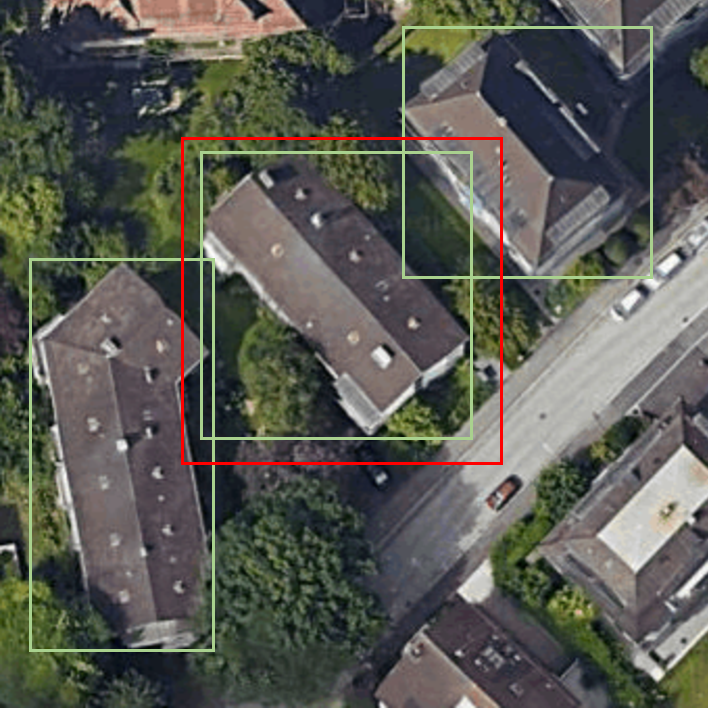
\includegraphics[width=\figfigfigfig\textwidth]{3-07-0.pdf}}
	\subbottom[Natural\label{fig:natanchor1}]
		{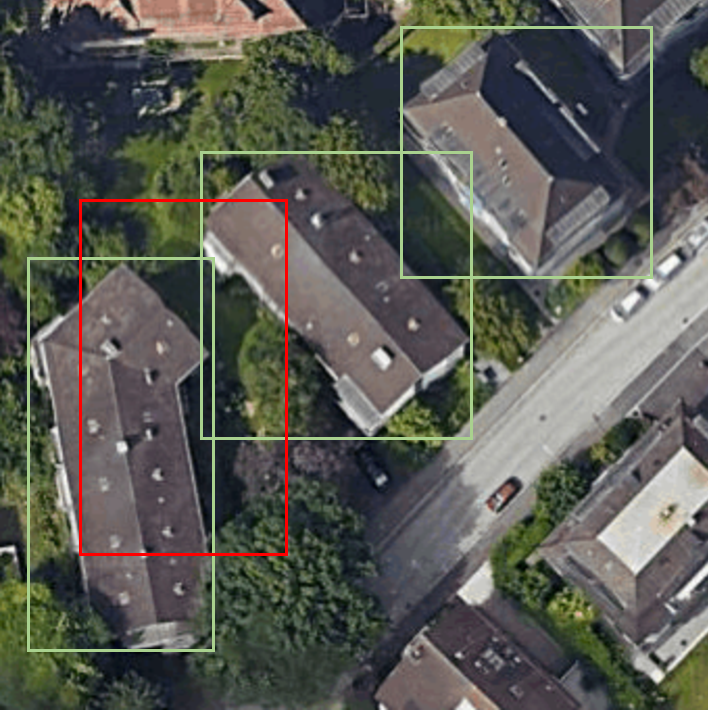
\includegraphics[width=\figfigfigfig\textwidth]{3-07-1.pdf}}
	\subbottom[Natural\label{fig:natanchor2}]
		{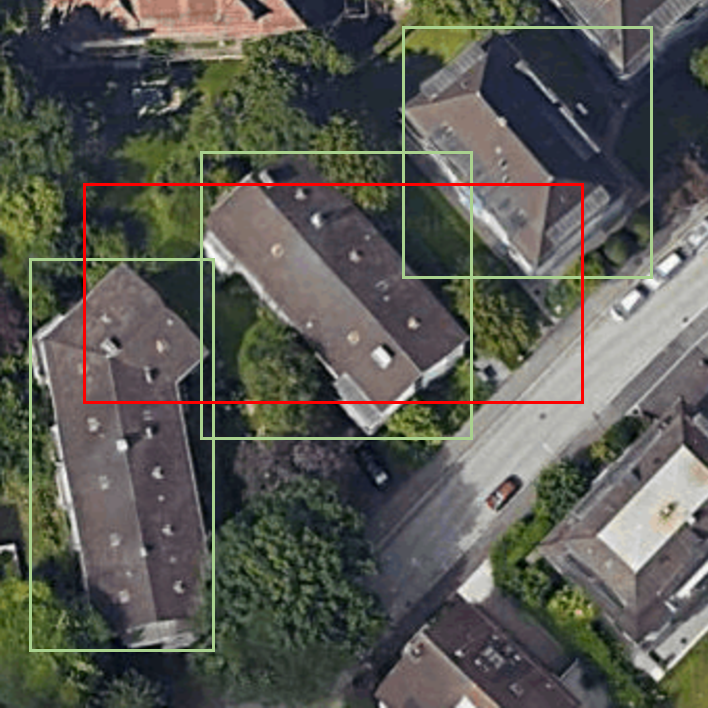
\includegraphics[width=\figfigfigfig\textwidth]{3-07-2.pdf}}
	\subbottom[Negative\label{fig:neganchor}]
		{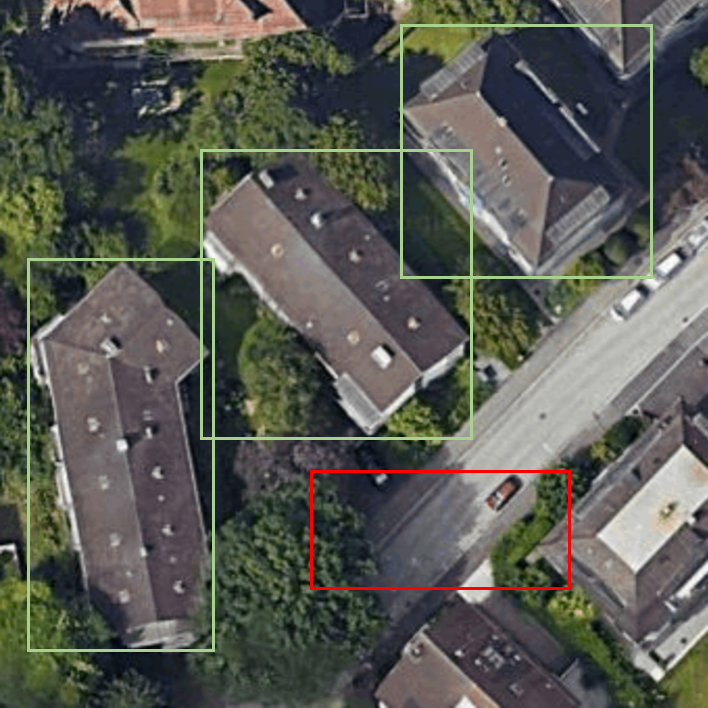
\includegraphics[width=\figfigfigfig\textwidth]{3-07-3.pdf}}
    \caption[Example anchors in image with multiple RoIs]{Example anchors in image  with multiple RoIs. (a)--(d) show four possible anchors in an image with  with multiple RoIs, with each showing one anchor. The red and light green rectangles refer to anchors and ground truth bounding boxes respectively. The polarities of these anchors are also shown, using the typical threshold.}
	\label{fig:eganchor}
\end{figure}